\section{Balmer-Serie}\label{sec:balmer}
\subsection{Versuchsaufbau und -durchführung}\label{subsec:balmer_durchfuhrung}
In diesem Versuchsteil wird die Balmer-Serie des Wasserstoffs samt Isotopieaufspaltung mithilfe eines Reflexionsgitters ausgemessen.
Dafür werden zunächst die Optikelemente nach \cref{fig:balmer_aufbau} aufgebaut und auf eine Höhe ausgerichtet.
\begin{figure}[H]
	\centering
	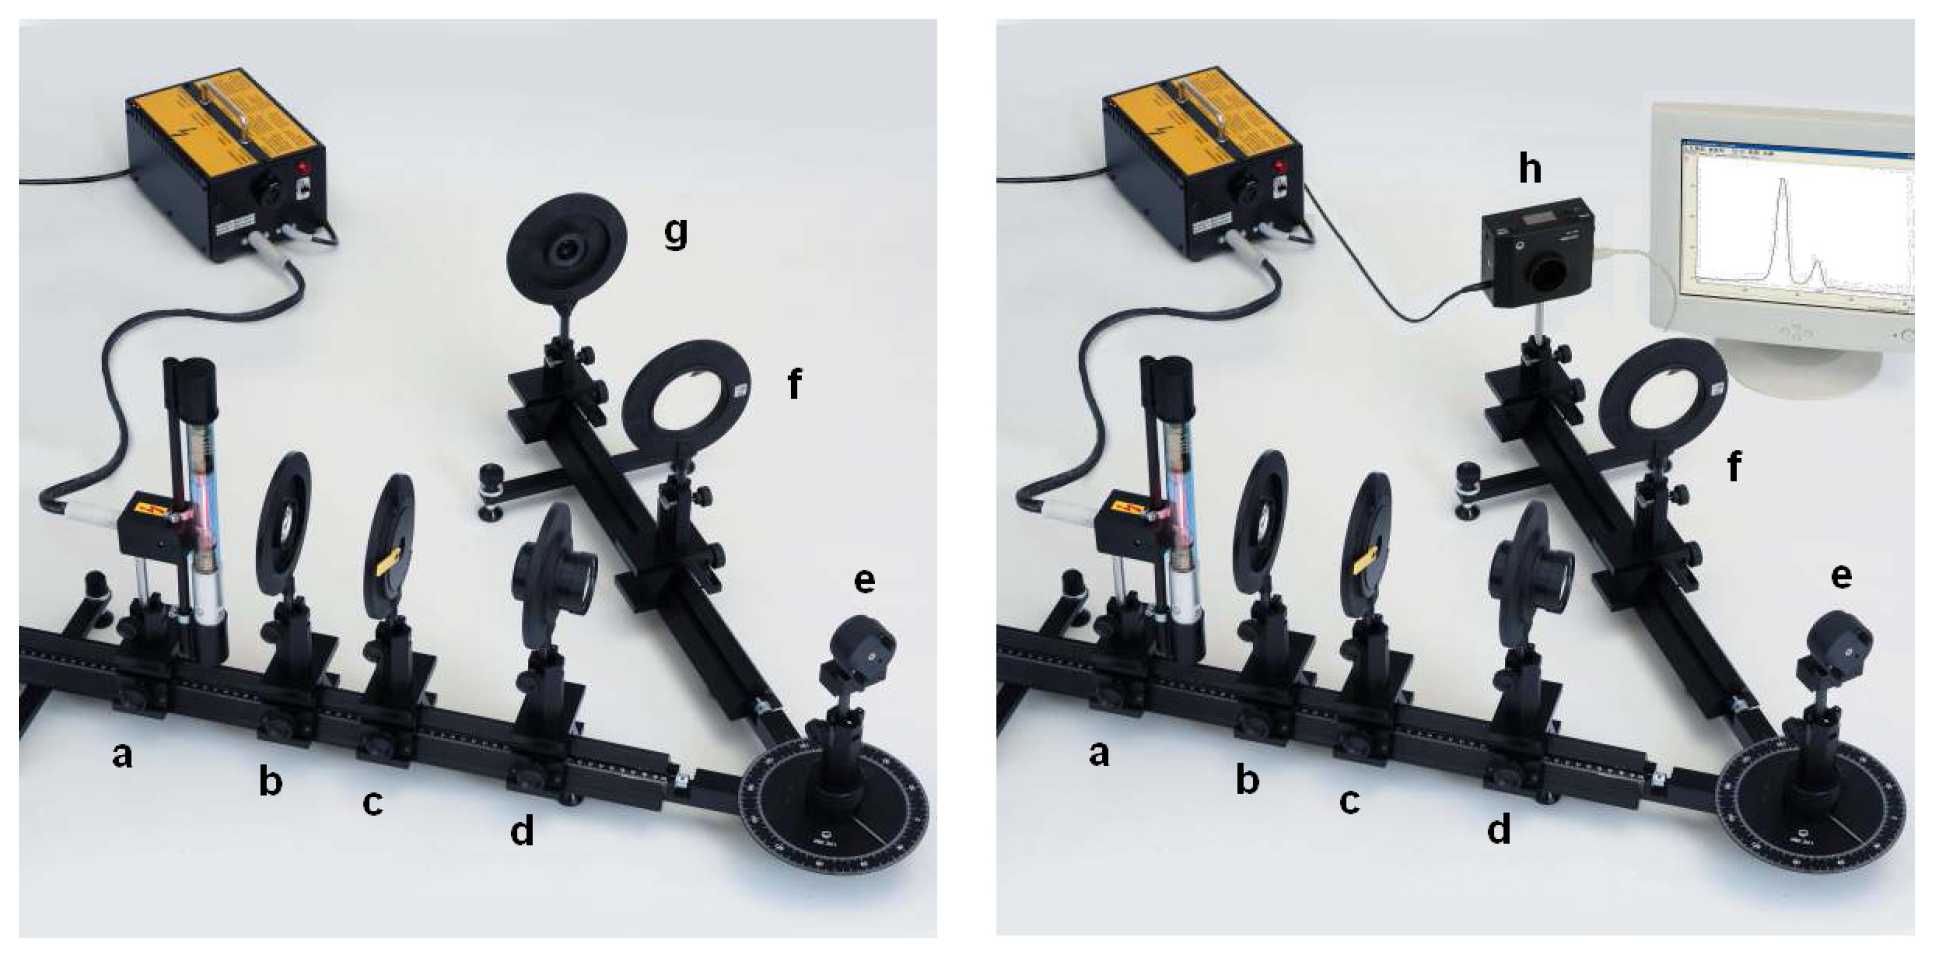
\includegraphics[width=0.8\linewidth]{../figs/balmer_aufbau}
	\caption{Versuchsaufbau zur Vermessung der Balmer-Serie mit Okular (links) und mit CCD-Kamera (rechts) \cite{skript}}
	\label{fig:balmer_aufbau}
\end{figure} Die verwendeten Optikelemente sind:
\begin{itemize}
    \item[\textbf{a}] Balmer-Lampe, deuteriert
    \item[\textbf{b}] Linse, $f = \SI{50}{\milli \meter}$
    \item[\textbf{c}] Verstellbarer Spalt, schräge Flanken zur Lichtquelle
    \item[\textbf{d}] Projektionsobjektiv, $f = \SI{150}{\milli \meter}$
    \item[\textbf{e}] Holographisches Gitter
    \item[\textbf{f}] Linse, $f = \SI{300}{\milli \meter}$
    \item[\textbf{g}] Okular mit Strichskala
    \item[\textbf{h}] CCD-Kamera      
\end{itemize}
Für eine erfolgreiche Durchführung ist eine möglichst exakte Justierung des Versuchsaufbaus notwendig. Dafür wird zuerst die Hg-Spektrallampe eingesetzt, welche
dann mithilfe der Linse mit der Brennweite $f = \SI{50}{\milli \meter}$ auf den Spalt abgebildet wird. Anschließend wird das Projektionsobjektiv im Brennweitenabstand
$f = \SI{150}{\milli \meter}$ hinter dem Spalt positioniert, sodass hinter dem Projektionsobjektiv paralleles Licht für das Reflexionsgitter zur Verfügung steht.\par
Die Säule des Drehgelenks wird so gedreht, dass der Zeiger auf \SI{0}{\degree} der umliegenden Skala weist. Nachdem die Säule mit einer Rändelschraube fixiert ist,
wird das Reflexionsgitter senkrecht  eingesetzt, sodass Licht auf den Spalt reflektiert wird. Damit für das Reflexionsgitter auch tatsächlich paralleles Licht
zur Verfügung steht, muss der Spalt ins Unendliche abgebildet werden, was durch die vorherige Positionierung des Projektionsobjektivs nicht unbedingt erreicht wird.
Daher wird nun das Projektionsobjektiv etwas verschoben, bis ein scharfes Bild des Spaltes neben dem Spalt zu erkennen ist. Dann wird das Gitter so ausgerichtet,
dass das Bild des Spaltes genau im Spalt selbst liegt.\par
Der Winkel der beiden optischen Bänke wird auf $\omega_{\mathrm{B}} = \SI{140,0(5)}{\degree}$ eingestellt.
Die Unsicherheit wird hier auf $\delta \omega_{\mathrm{B}} = \SI{0,5}{\degree}$ abgeschätzt, da der Winkel mindestens bis auf diese Genauigkeit abgelesen werden kann.
Diese Einstellung wird für die gesamte Versuchsdurchführung beibehalten.
Auf der anderen optischen Bank wird das Okular am Ende der Schiene eingesetzt und so eingestellt, dass die Strichskala gut ablesbar ist. Abschließend wird die Linse
mit der Brennweite $f = \SI{300}{\milli \meter}$ vor das Okular gestellt, sodass dies einem Fernrohraufbau entspricht. Bei diesem Versuchsaufbau wird das Reflexionsgitter
verwendet, um die diskreten Spektrallinien, aus denen sich das Licht einer Spektrallampe (Hg-Spektrallampe und Balmer-Lampe) zusammensetzt, nebeneinander abzubilden.
Das Reflexionsgitter wird mit parallelem Licht bestrahlt, sodass die Gittergleichung für die erste Beugungsordnung
\begin{equation}\label{eq:gittergleichung}
    \lambda = g (\sin(\alpha) + \sin(\beta))
\end{equation} gilt. So gibt es nämlich für jede Wellenlänge $\lambda$ bei einem fixierten Einfallswinkel $\alpha$ einen anderen Ausfallswinkel $\beta$, sodass die Spektrallinien
nebeneinander beobachtet werden können. Eine detaillierte Herleitung dieser Formel ist in \cite{balmer_handblatt} zu finden.\newline
\indent Da der vom Hersteller angegebene Wert für die Gitterkonstante nicht genau ist, wird die Gitterkonstante zunächst mithilfe der Hg-Spektrallampe bestimmt,
deren wichtigsten Spektrallinien und zugehörigen Wellenlängen bekannt sind. Für jede dieser Spektrallinien wird das Gitter so gedreht, dass die Linie auf der Strichskala
des Okulars zu beobachten ist. Es wird der Winkel des Gitter $\omega_{\mathrm{G}}$ abgelesen. Der Zusammenhang zwischen den gemessenen Winkeln $\omega_{\mathrm{B}}$ und $\omega_{\mathrm{G}}$
und dem Ein- bzw. Ausfallswinkel des Lichtes folgt aus \cref{fig:winkel_am_aufbau}.
\begin{figure}[H]
	\centering
	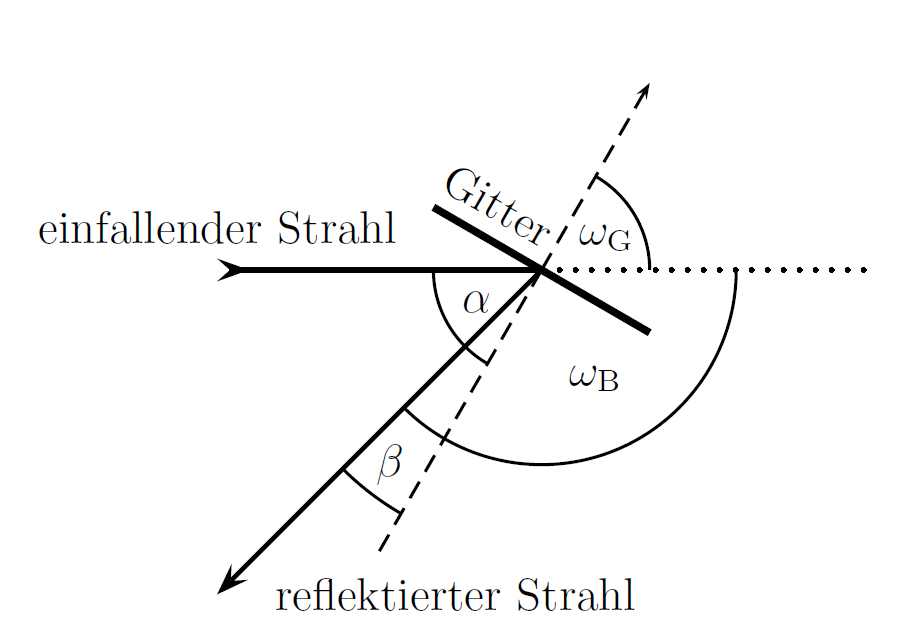
\includegraphics[width=0.5\linewidth]{../figs/winkel_am_aufbau.png}
	\caption{Winkel am Aufbau \cite{skript}}
	\label{fig:winkel_am_aufbau}
\end{figure} Aus geometrischen Überlegungen folgen die Relationen:
\begin{align}\label{eq:winkel}
    \alpha &= \omega_{\mathrm{G}} \\
    \beta &= \omega_{\mathrm{G}} + \omega_{\mathrm{B}} - \SI{180}{\degree} .
\end{align} Durch die Kenntnis der Wellenlänge einer Linie und die zugehörigen Winkel $\alpha$ und $\beta$ kann dann mithilfe der Gittergleichung \ref{eq:gittergleichung}
die Gitterkonstante des verwendeten Reflexionsgitters bestimmt werden. Um anschließend das Spektrum der Balmer-Lampe zu vermessen, wird diese anstelle der Hg-Spektrallampe eingesetzt.
Erneut werden die Winkel des Reflexionsgitters für die einzelnen Spektrallinien gemessen. Mithilfe der bereits bestimmten Gitterkonstante können dann die Wellenlängen der
einzelnen Spektrallinien der Balmer-Lampe ermittelt werden. Außerdem wird die Isotopieaufspaltung beobachtet, da die Balmer-Lampe mit Dampf aus deuteriertem und normalem Wasserstoff
(Verhältnis  ca. 1:2) gefüllt ist.\par
Abschließend wird das Okular durch eine CCD-Kamera ausgetauscht. Die CCD-Kamera wird mit einem Computer verbunden, sodass die
Spektrallinien der Balmer-Lampe mit dem Programm \enquote{VideoCom-Intensitäten} aufgezeichnet werden können. Dies eignet sich später zu einer genaueren Bestimmung
der Isotopieaufspaltung. Das Programm berechnet aus der Pixelkoordinate $p$, die von 0 bis 2047 läuft, den Winkel $\beta$ über
\begin{equation*}
    \beta = \arctan(\frac{(1024 - p) \cdot \SI{0,014}{\milli \meter}}{f}) .
\end{equation*}

\subsection{Messung}\label{subsec:balmer_messung}
Zuerst wird der Winkel $\omega_{\mathrm{G}}$ (bei fixiertem Winkel $\omega_{\mathrm{B}} = \SI{140,0(5)}{\degree}$) für die verschiedenen Spektrallinien der
Hg-Spektrallampe gemessen. Dafür wird die Säule mit dem eingesetzten Reflexionsgitter gedreht, bis die erste sichtbare Linie zu beobachten ist. Um die Linie
aufzufinden, wird der Spalt erst etwas weiter geöffnet und anschließend wieder verkleinert. Das Projektionsobjektiv muss für jede Spektrallinie leicht verschoben werden, sodass
diese scharf zu erkennen ist. Bei der Messung ergibt sich die Schwierigkeit, dass manche Spektrallinien so nah aneinander liegen, dass für diese der gleiche Winkel
$\omega_{\mathrm{G}}$ abgelesen wird. Um dennoch eine Winkeldifferenz für diese Linien messen zu können, wird zusätzlich die Strichskala des Okulars benutzt. Diese Strichskala
hat eine Länge von \SI{10}{\milli \meter} mit einer Teilung von \SI{0,1}{\milli \meter}. Es wird stets so vorgegangen, dass der Winkel $\omega_{\mathrm{G,gemessen}}$ für eine bestimmte
Spektrallampe auf der Kreisskala exakt eingestellt wird. Um später aber den tatsächlichen Winkel für diese Spektrallinie zu erhalten, wird zusätzlich über das Okular
die Abweichung $d$ von der Mitte der Strichskala aus gemessen (später folgt die entsprechende Winkelabweichung über die Brennweite der Linse vor dem Okular).\par
In der Auswertung werden diese Messgrößen miteinander verrechnet, um möglichst genaue Werte für den Ein- und Ausfallswinkel zu erhalten. Auch wenn beide Messgrößen einen
eigenen Ablesefehler ($\delta \omega_{\mathrm{G,gemessen}}$ und $\delta d$) haben, wird später in der Auswertung die Unsicherheit des tatsächlichen Gitterwinkels zu $\delta \omega_{\mathrm{G}} = \SI{0,5}{\degree}$
abgeschätzt, da die Unsicherheit der resultierenden Winkelabweichung, welche sich aus $d$ berechnet, extrem klein ist und dann schon in der festgesetzten Unsicherheit $\delta \omega_{\mathrm{G}} = \SI{0,5}{\degree}$
enthalten ist. Ohnehin gibt es hier eine systematische Unsicherheit bei der Messung von $\omega_{\mathrm{G,gemessen}}$, da das Gitter nicht perfekt in die Halterung platziert werden kann.
Allerdings gibt es hier keine Möglichkeit, diese systematische Unsicherheit abzuschätzen. Aber auch diese ist gegenüber \SI{0,5}{\degree} klein, weshalb die spätere
Fehlerabschätzung $\delta \omega_{\mathrm{G}} = \SI{0,5}{\degree}$ sinnvoll ist.
\begin{table}[H]
    \centering
    \caption{Gemessene Spektrallinien der Hg-Spektrallampe}
    \begin{tabular}{c|c|c|c}
        Farbe & $\lambda_{\mathrm{Hg}}$ / \unit{\nano \meter} & $\omega_{\mathrm{G,gemessen}}$ / \unit{\degree} & $d$ / \unit{\milli \meter} \\
        \hline
        violett & 404,656 & 52 & $+$0,0 \\
        violett & 407,783 & 52 & $+$2,0 \\
        violett & 410,805 & 52 & $+$4,0 \\
        violett & 433,922 & 55 & $-$2,7 \\
        violett & 434,749 & 55 & $-$2,1 \\
        blau & 435,833 & 55 & $-$1,5 \\
        türkis & 491,607 & 60 & $+$0,0 \\
        grün & 546,074 & 65 & $+$1,8 \\
        gelb & 576,960 & 69 & $-$1,6 \\
        gelb & 579,066 & 69 & $+$0,0 \\
        rot & 623,440 & 72 & $-$1,0 \\
        rot & 671,643 & 72 & $+$3,0 \\
        rot & 690,752 & 74 & $+$0,0
    \end{tabular}\label{tab:spektrallinien_hg}
\end{table} Die aufgenommenen Messwerte sind in \cref{tab:spektrallinien_hg} zu finden, wobei die Wellenlängen der Versuchsanleitung \cite{skript} entnommen sind.
Später in der Auswertung werden $\omega_{\mathrm{G,gemessen}}$ und $d$ zu $\omega_{\mathrm{G}}$ mit der abgeschätzten Unsicherheit $\delta \omega_{\mathrm{G}} = \SI{0,5}{\degree}$ verrechnet.
In \cref{tab:spektrallinien_hg} ist die Messgröße $d$ entweder mit einem positiven oder negativen Vorzeichen versehen, je nachdem ob die beobachtete Spektrallinie links oder rechts
von der Mitte der Strichskala zu sehen war.\newline
\indent Nun wird die Hg-Spektrallampe durch die Balmer-Lampe ersetzt. Der Aufbau muss etwas nachjustiert werden und dann können die Messwerte analog aufgenommen werden.
Da die einzelnen Spektrallinien der Balmer-Lampe im Vergleich zu der Hg-Spektrallampe wesentlich weiter auseinander liegen, wird hier lediglich der Winkel des Gitters
an der Kreisskala mit einer Unsicherheit von $\delta \omega_{\mathrm{G}} = \SI{0,5}{\degree}$ abgelesen. Hier ist nun auch die Isotopieaufspaltung zu beobachten, welche durch die
Messgröße $d$ (Unsicherheit abgeschätzt auf $\delta d = \SI{0,1}{\milli \meter}$) auf der Strichskala gemessen wird. Insgesamt können drei Linien der Balmer-Serie (inklusive Isotopieaufspaltung) gut erkannt werden. Bei der violetten Linie konnte leider keine Isotopieaufspaltung aufgelöst werden. Die aufgenommenen Messwerte sind in \cref{tab:spektrallinien_balmer}
zu erkennen.
\begin{table}[H]
    \centering
    \caption{Gemessene Spektrallinien der Balmer-Lampe}
    \begin{tabular}{c|c|c|c}
        Farbe & $\omega_{\mathrm{G}}$ / \unit{\degree} & $d$ / \unit{\milli \meter} \\
        \hline
        rot & 78,0 & 0,2 \\
        türkis & 59,0 & 0,1 \\
        violett & 54,0 & nicht erkennbar
    \end{tabular}\label{tab:spektrallinien_balmer}
\end{table} Abschließend werden noch diese drei Spektrallinien bei jeweils gleichem Gitterwinkel mit der CCD-Kamera und dem zugehörigen Computer-Programm aufgenommen 
(die Daten sind hier vorzufinden: \url{https://uni-bonn.sciebo.de/s/dkCZbAXN5Exv807}).
Bei jeder Messung muss das Projektionsobjektiv leicht verschoben werden, um die jeweilige Spektrallinie inklusive Isotopieaufspaltung möglichst genau aufzeichnen zu können.
Es wird darauf geachtet, dass die Säule mit dem Reflexionsgitter möglichst so gedreht wird, dass die jeweilige Spektrallinie bei \SI{0}{\degree} abegebildet wird.
Dies war leider aufgrund der hohen Empfindlichkeit nicht immer möglich, was aber später in der Auswertung leicht korrigiert werden kann.

\subsection{Auswertung}\label{subsec:balmer_auswertung}
\subsubsection{Bestimmung der Gitterkonstanten}\label{subsubsec:gitterkonstante}
\footnote[1]{Bei diesem Versuchsteil werden Unsicherheiten stets mit einem $\delta$ gekennzeichnet, da das $\Delta$ bereits für viele andere verwendete Größen reserviert ist.}Mithilfe der Gittergleichung \ref{eq:gittergleichung} kann für jede Linie der Hg-Spektrallampe die Gitterkonstante ausgerechnet werden. Dafür werden Ein- und Ausfallswinkel
benötigt, welche sich mit \cref{eq:winkel} berechnen lassen. Hierfür wird zunächst Folgendes benötigt:
\begin{equation*}
    \omega_{\mathrm{G}} = \omega_{\mathrm{G,gemessen}} + \omega_{\mathrm{d}} \approx \omega_{\mathrm{G,gemessen}} + \frac{d}{f} \cdot \frac{\SI{180}{\degree}}{\pi} = \omega_{\mathrm{G,gemessen}} + \frac{d}{\SI{300}{\milli \meter}} \cdot \frac{\SI{180}{\degree}}{\pi} ,
\end{equation*} wobei die Kleinwinkelnäherung $\omega_{\mathrm{d}} [\unit{\radian}] \approx \frac{d}{f}$ (hier ist $f = \SI{300}{\milli \meter}$ die Brennweite der Linse vor dem Okular) verwendet wurde.
Wie schon zuvor erwähnt, wird hier die Unsicherheit sinnvoll auf $\delta \omega_{\mathrm{G}} = \SI{0,5}{\degree}$ abgeschätzt. Für die Unsicherheit von Ein- und Ausfallswinkel gilt:
\begin{equation*}
    \delta \alpha = \delta \omega_{\mathrm{G}} , \quad \delta \beta = \sqrt{(\delta \omega_{\mathrm{G}})^2 + (\delta \omega_{\mathrm{B}})^2} .
\end{equation*} Die Gitterkonstante wird durch $g = \frac{\lambda}{\sin(\alpha) + \sin(\beta)}$ berechnet, wobei die zugehörige Unsicherheit durch
\begin{align*}
    \delta g &= \sqrt{\left(\pdv{g}{\alpha} \delta \alpha\right)^2 + \left(\pdv{g}{\beta} \delta \beta\right)^2} \\
    &= \sqrt{\left(\frac{\lambda}{(\sin(\alpha) + \sin(\beta))^2} \cos(\alpha) \delta \alpha\right)^2 + \left(\frac{\lambda}{(\sin(\alpha) + \sin(\beta))^2} \cos(\beta) \delta \beta\right)^2} \\
    &= \frac{g}{\sin(\alpha) + \sin(\beta)} \sqrt{(\cos(\alpha) \delta \alpha)^2 + (\cos(\beta) \delta \beta)^2}
\end{align*} gegeben ist. Die ermittelten Werte für die Gitterkonstante für jede gemessene Hg-Spektrallinie sind in \cref{tab:gitterkonstanten} dargestellt.
\begin{table}[H]
    \centering
    \caption{Bestimmung der Gitterkonstante für jede gemessene Hg-Spektrallinie}
    \begin{tabular}{c|c|c|c|c}
        $\lambda_{\mathrm{Hg}}$ / \unit{\nano \meter} & $(\alpha \pm 0,5)$ / \unit{\degree} & $(\beta \pm 0,8)$ / \unit{\degree} & $g$ / \unit{\nano \meter} & $\delta g$ / \unit{\nano \meter} \\
        \hline
        404,656 & 52,0 & 12,0 & 406 & 6 \\
        407,783 & 52,4 & 12,4 & 405 & 6 \\
        410,805 & 52,8 & 12,8 & 404 & 6 \\
        433,922 & 54,5 & 14,5 & 408 & 5 \\
        434,749 & 54,6 & 14,6 & 407 & 5 \\
        435,833 & 54,7 & 14,7 & 407 & 5 \\
        491,607 & 60,0 & 20,0 & 407 & 5 \\
        546,074 & 65,3 & 25,3 & 408 & 4 \\
        576,960 & 68,7 & 28,7 & 409 & 4 \\
        579,066 & 69,0 & 29,0 & 408 & 4 \\
        623,440 & 71,8 & 31,8 & 422 & 4 \\
        671,643 & 72,6 & 32,6 & 450 & 4 \\
        690,752 & 74,0 & 34,0 & 454 & 4
    \end{tabular}\label{tab:gitterkonstanten}
\end{table} Besonders die drei letzten Werte für die Gitterkonstante unterscheiden sich stark von den restlichen Werten. Der Grund dafür liegt darin, dass diese Linien
aufgrund der vergleichsweise geringen Intensität sehr schwierig zu beobachten und auf der Strichskala scharf zu stellen waren. Vermutlich wurden dann sehr ungenaue Messwerte
aufgenommen. Daher werden diese drei letzten Spektrallinien für die weitere Auswertung zur Bestimmung der Gitterkonstanten nicht berücksichtigt.\newline
\indent Um einen Wert für die Gitterkonstante aus allen Messwerten zu gewinnen, wird eine Geraden-Anpassung durchgeführt. Die Geraden-Gleichung ist durch
\begin{equation*}
    y = \sin(\alpha) + \sin(\beta) = a \lambda = \frac{1}{g} \lambda
\end{equation*} gegeben. Für die Unsicherheit der $y$-Werte gilt $\delta y = \sqrt{(\cos(\beta) \delta \alpha)^2 + (\cos(\beta) \delta \beta)^2}$.
Die Werte für die Geraden-Anpassung sind in \cref{tab:geraden_fit_gitterkonstante} eingetragen und die zugehörige graphische Darstellung ist in \cref{fig:geraden_fit_gitterkonstante}
zu sehen.
\begin{table}[H]
    \centering
    \caption{Werte der Geraden-Anpassung zur Bestimmung der Gitterkonstanten}
    \begin{tabular}{c|c|c}
        $\lambda_{\mathrm{Hg}}$ / \unit{\nano \meter} & $y$ & $\delta y$\\
        \hline
        404,656 & 0,996 & 0,013 \\
        407,783 & 1,007 & 0,013 \\
        410,805 & 1,017 & 0,013 \\
        433,922 & 1,064 & 0,013 \\
        434,749 & 1,067 & 0,013 \\
        435,833 & 1,070 & 0,013 \\
        491,607 & 1,208 & 0,013 \\
        546,074 & 1,337 & 0,012 \\
        576,960 & 1,412 & 0,012 \\
        579,066 & 1,418 & 0,012
    \end{tabular}\label{tab:geraden_fit_gitterkonstante}
\end{table}
\begin{figure}[H]
	\centering
	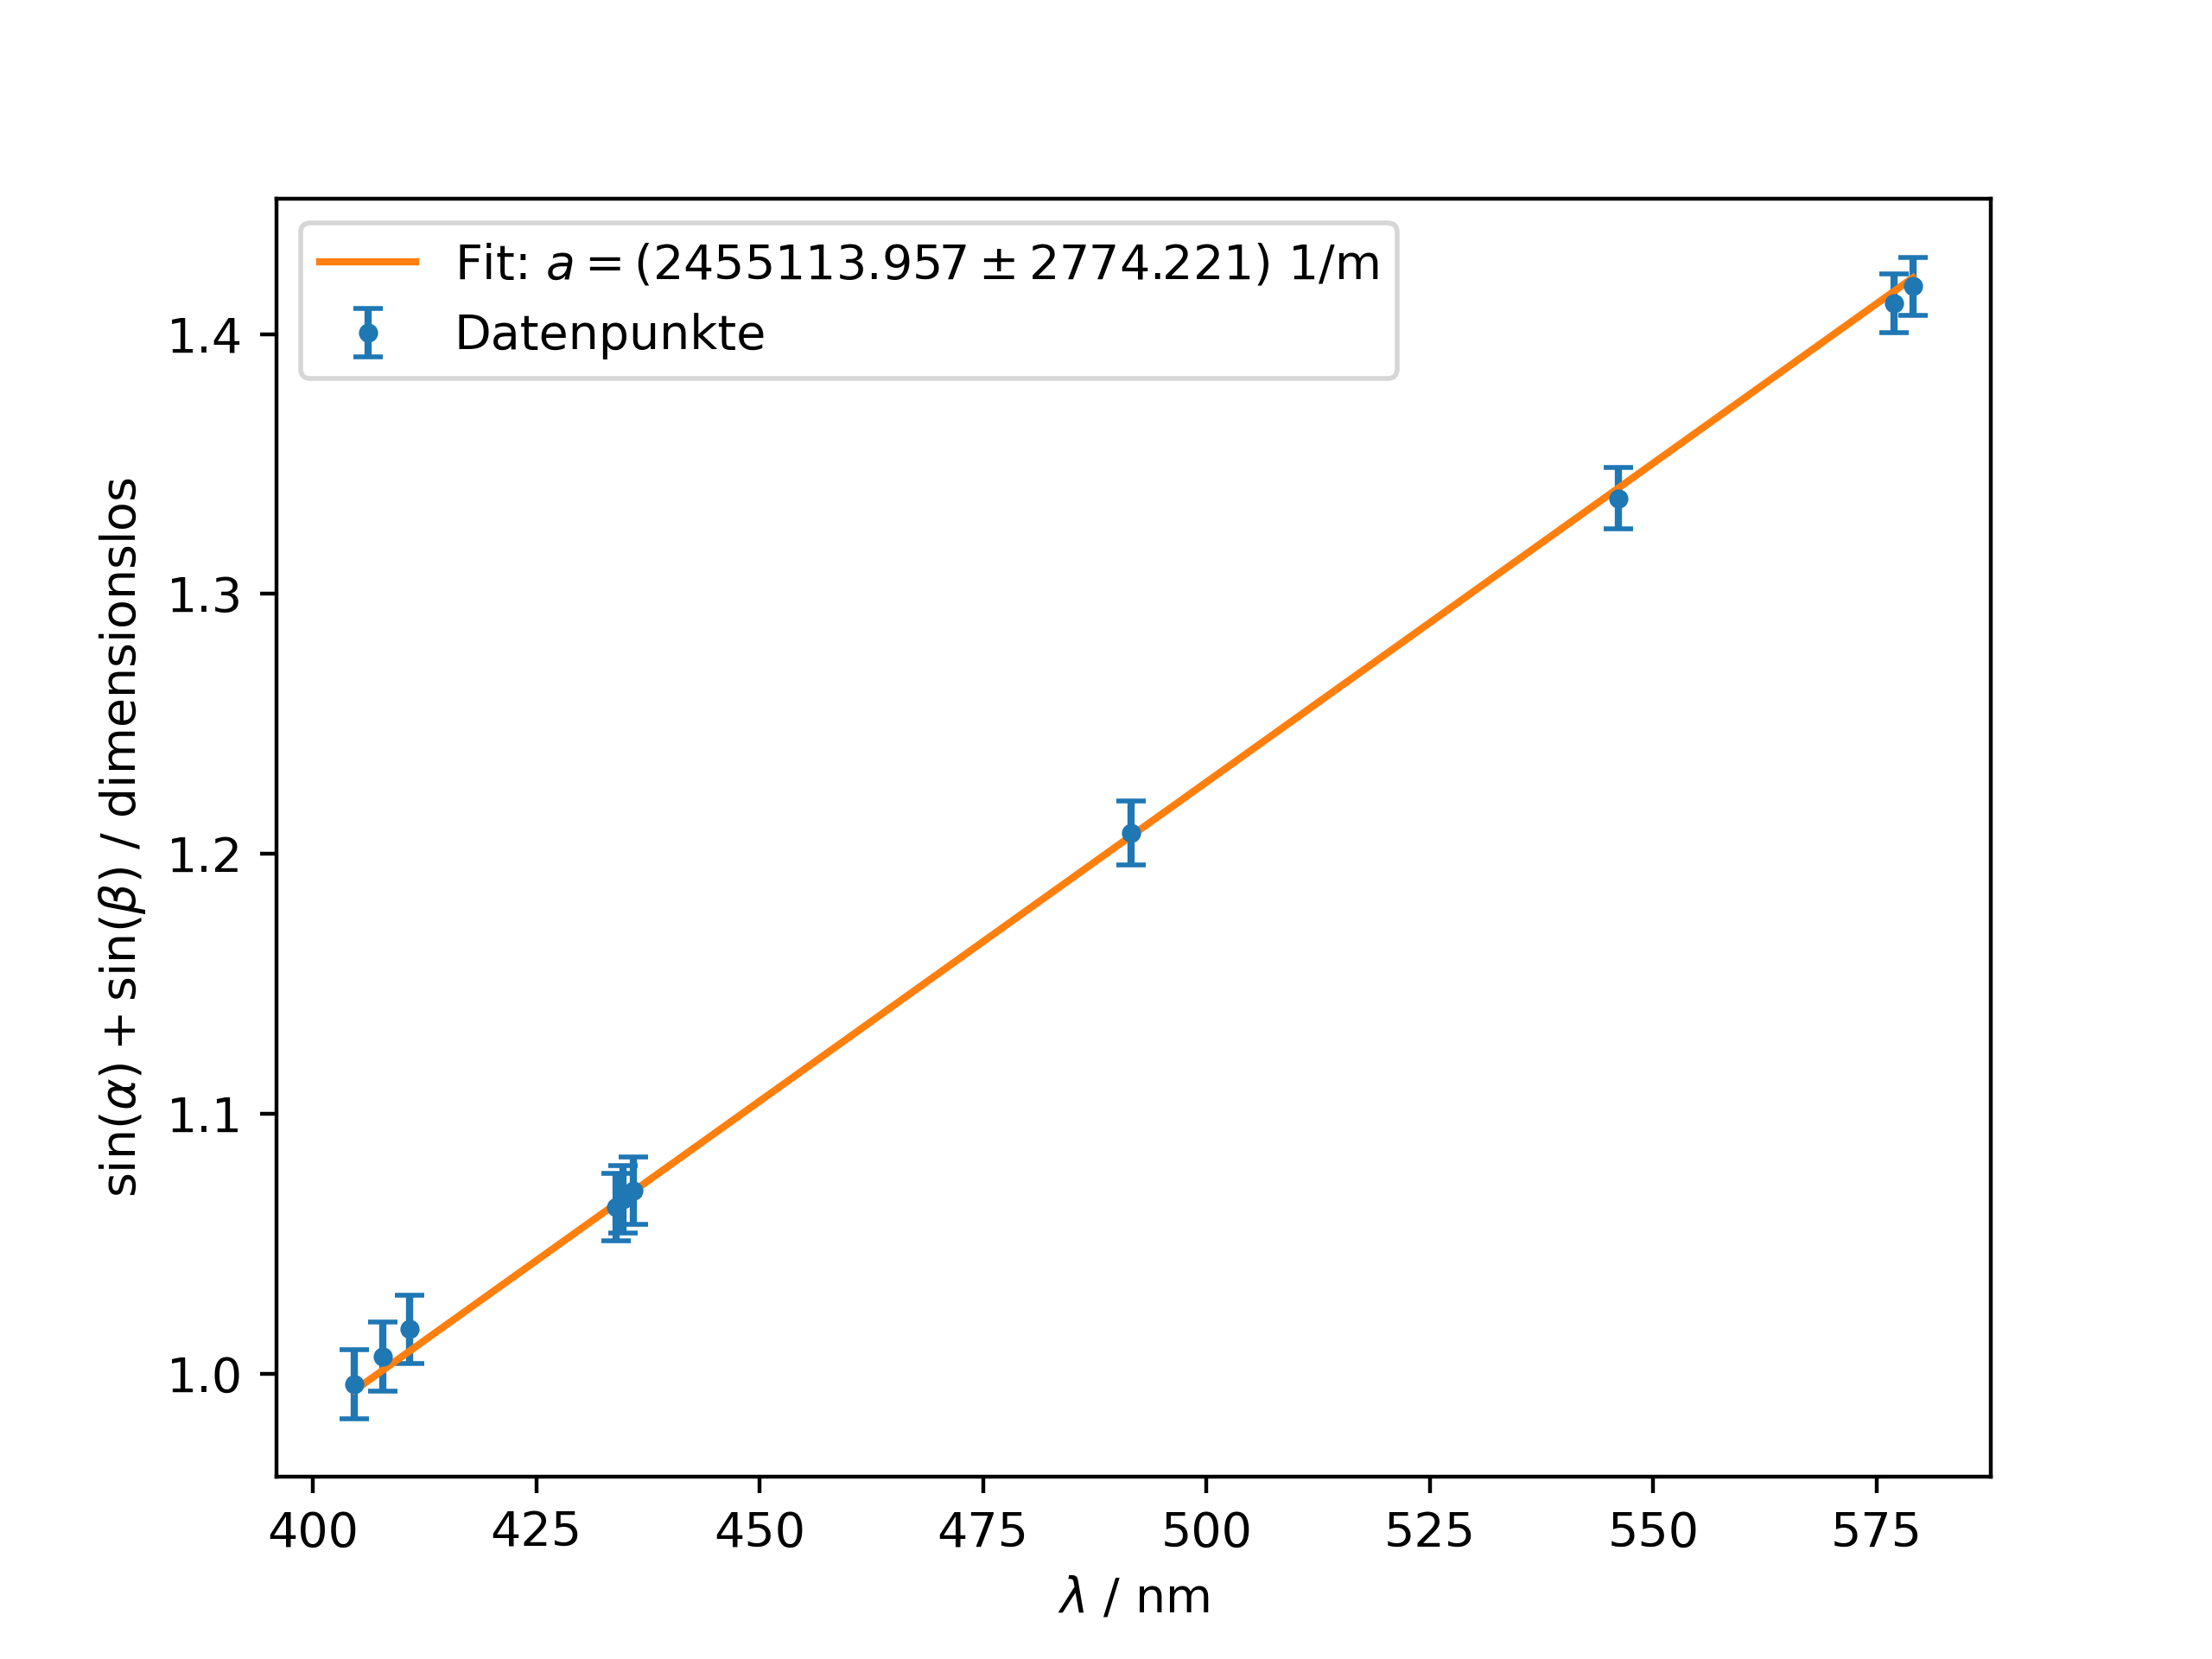
\includegraphics[width=0.8\linewidth]{../figs/gitterkonstante_fit.png}
	\caption{Geraden-Anpassung zur Bestimmung der Gitterkonstanten}
	\label{fig:geraden_fit_gitterkonstante}
\end{figure} Mit $\chi^2 = 0.00016$ kann von einer gelungenen Anpassung der Gerade an die Datenpunkte gesprochen werden. Die Gitterkonstante ergibt sich nun aus
dem Anpassungsparameter $a = \SI{2,4551(28)e6}{\frac{1}{\meter}}$ gemäß $g = \frac{1}{a}$ mit der Unsicherheit $\delta g = \frac{\delta a}{a^2}$:
\begin{equation}\label{eq:gitterkonstante}
    g = \SI{407(5)}{\nano \meter} .
\end{equation} Da bei dem verwendeten Reflexionsgitter keine Herstellerangabe zu der Gitterkonstanten vorhanden war, kann an dieser Stelle kein Vergleich mit einem
Literaturwert durchgeführt werden. Jedoch zeigt die Güte der Geraden-Anpassung, dass ein gutes Ergebnis erzielt wurde. Der in \cref{eq:gitterkonstante} dargestellte
Wert für die experimentell bestimmte Gitterkonstante wird nun für die gesamte weitere Auswertung verwendet.

\subsubsection{Bestimmung der Balmerlinien}\label{subsubsec:balmerlinien}
Mithilfe der soeben bestimmten Gitterkonstanten können nun die Wellenlängen zu den vermessenen Spektrallinien der Balmer-Lampe ermittelt werden. Erneut werden
Ein- und Ausfallswinkel gemäß \cref{eq:winkel} berechnet. Die Unsicherheiten sind durch $\delta \alpha = \delta \omega_{\mathrm{G}} = \SI{0,5}{\degree}$
und $\delta \beta = \sqrt{(\delta \omega_{\mathrm{G}})^2 + (\delta \omega_{\mathrm{B}})^2} = \SI{0,8}{\degree}$ gegeben. Dann können die Wellenlängen zu den einzelnen
Spektrallinien mit der Gittergleichung \ref{eq:gittergleichung} und der zugehörigen Unsicherheit
\begin{align*}
    \delta \lambda &= \sqrt{\left(\pdv{\lambda}{g} \delta g\right)^2 + \left(\pdv{\lambda}{\alpha} \delta \alpha\right)^2 + \left(\pdv{\lambda}{\beta} \delta \beta\right)^2} \\
    &= \sqrt{((\sin(\alpha) + \sin(\beta)) \delta g)^2 + (g \cos(\alpha) \delta \alpha)^2 + (g \cos(\beta) \delta \beta)^2}
\end{align*} berechnet werden. Die berechneten Werte können dann mit Literaturwerten verglichen werden, welche \cite{balmer_handblatt} entnommen sind und dann der entsprechenden
Spektrallinie zugeordnet werden. Dies ist in \cref{tab:wellenlangen_balmer} dargestellt.
\begin{table}[H]
    \centering
    \caption{Experimentell bestimmte Wellenlängen der Balmer-Spektrallinien}
    \begin{tabular}{c|c|c|c|c|c}
        Spektrallinie & ($\alpha \pm \SI{0,5}{\degree}$) / \unit{\degree} & ($\beta \pm \SI{0,8}{\degree}$) / \unit{\degree} & $\lambda$ / \unit{\nano \meter} & $\delta \lambda$ / \unit{\nano \meter} & $\lambda_{\mathrm{Lit}}$ / \unit{\nano \meter} \\
        \hline
        $\mathrm{H_{\alpha}}$ & 78,0 & 38,0 & 649 & 5 & 656,28 \\
        $\mathrm{H_{\beta}}$ & 59,0 & 19,0 & 482 & 6 & 486,13 \\
        $\mathrm{H_{\gamma}}$ & 54,0 & 14,0 & 428 & 6 & 434,05
    \end{tabular}\label{tab:wellenlangen_balmer}
\end{table} Die Literaturwerte der Wellenlängen liegen für die einzelnen Linien in der 1--2-$\sigma$-Umgebung der experimentell bestimmten Wellenlängen, womit hier gute Ergebnisse erzielt wurden.\newline
\indent Nun wird die Isotopieaufspaltung (repräsentiert durch den Wellenlängenunterschied $\Delta \lambda$ zwischen der jeweiligen Spektrallinie des reinen Wasserstofffs und der entsprechenden
Spektrallinie des Deuteriums) bestimmt. Mithilfe von \cref{eq:gittergleichung} ergibt sich zunächst für $\Delta \lambda$:
\begin{equation}\label{eq:isotopieaufspaltung}
    \Delta \lambda = \pdv{\lambda}{\beta} \Delta \beta = g \cos(\beta) \Delta \beta .
\end{equation} Für die Unsicherheit gilt:
\begin{align*}
    \delta (\Delta \lambda) &= \sqrt{\left(\pdv{(\Delta \lambda)}{g} \delta g\right)^2 + \left(\pdv{(\Delta \lambda)}{\beta} \delta \beta\right)^2 + \left(\pdv{(\Delta \lambda)}{(\Delta \beta)} \delta (\Delta \beta)\right)^2} \\
    &= \sqrt{(\cos(\beta) \Delta \beta \delta g)^2 + (g \sin(\beta) \Delta \beta \delta \beta)^2 + (g \cos(\beta) \delta (\Delta \beta))^2} .
\end{align*} Außerdem berechnet sich die Winkelaufspaltung mit einer Kleinwinkelnäherung nach $\Delta \beta \approx \frac{d}{f}$ (bei den weiteren Berechnungen wird
eine Umrechnung in \unit{\degree} vorgenommen). Entsprechend berechnet sich die Unsicherheit gemäß $\delta (\Delta \beta) = \frac{\delta d}{f}$. Die Ergebnisse
sind in \cref{tab:aufspaltung_balmer} dargestellt, wobei keine Isotopieaufspaltung zu der $\mathrm{H_{\mathrm{\gamma}}}$-Spektrallinie bestimmt werden kann, da
die entsprechende Winkelaufspaltung während der Versuchsdurchführung nicht auflösbar war. Eine noch präzisere Justierung des Versuchsaufbaus hätte möglicherweise
zu einer Verbesserung geführt. Dies war jedoch schwierig umzusetzen, da einige der verwendeten Optikelemente leicht verbogen waren und nicht perfekt aufeinander
abgestimmt werden konnten.
\begin{table}[H]
    \centering
    \caption{Mit dem Okular bestimmte Isotopieaufspaltung der Balmer-Spektrallinien}
    \begin{tabular}{c|c|c|c|c}
        Spektrallinie & ($\Delta \beta \pm \SI{0,019}{\degree}$) / \unit{\degree} & $\Delta \lambda$ / \unit{\nano \meter} & $\delta (\Delta \lambda)$ / \unit{\nano \meter} & $\Delta \lambda_{\mathrm{Lit}}$ / \unit{\nano \meter} \\
        \hline
        $\mathrm{H_{\alpha}}$ & 0,038 & 0,21 & 0,11 & 0,19 \\
        $\mathrm{H_{\beta}}$ & 0,019 & 0,13 & 0,11 & 0,14 \\
        $\mathrm{H_{\gamma}}$ & / & / & / & 0,09
    \end{tabular}\label{tab:aufspaltung_balmer}
\end{table} Die Literaturwerte für die Isotopieaufspaltung sind wieder \cite{balmer_handblatt} entnommen. Diese liegen wieder in der 1--2-$\sigma$-Umgebung der
experimentell bestimmten Werte, womit von einem guten Ergebnis gesprochen werden kann.\newline
\indent Nun wird die Isotopieaufspaltung anhand der mit der CCD-Kamera aufgenommenen Messwerte bestimmt. Dazu wird an diese Messwerte eine Überlagerung
zweier Gauß-Kurven angepasst (eigentliche Spektrallinie inklusive Isotopieaufspaltung), da das Intensitäts-Profil einer Spektrallinie gaußförmig erwartet wird.
Die Überlagerung zweier Gauß-Kurven (inklusive Offset $O$) ist gegeben durch:
\begin{equation*}
    f(\beta) = A_1 \exp(-\frac{(\beta - \beta_1)^2}{2 \sigma_1^2}) + A_2 \exp(-\frac{(\beta - \beta_2)^2}{2 \sigma_2^2}) + O .
\end{equation*} Bei der Aufnahme der Messwerte wurde das Ziel verfolgt, dass das Maximum der jeweiligen Balmer-Spektrallinie auf \SI{0}{\degree} abgebildet wird.
Aufgrund der Empfindlichkeit der Säule mit dem Gitter war dies jedoch nicht möglich. Daher werden die Messwerte für die Winkel in der Auswertung nun so verschoben, dass
das Maximum der jeweiligen Balmer-Spektrallinie trotzdem bei \SI{0}{\degree} zu sehen ist, da dies die weitere Auswertung dieses Versuchsteil erleichtert und auch
genauere Ergebnisse liefert. Für die Anpassung wird aus dem Python-Modul \enquote{scipy} die Funktion \enquote{Orthogonal distance regression} verwendet.
Für die mit der CCD-Kamera aufgenommenen Messwerte sind keine Unsicherheiten angegeben. Jedoch wird der Messfehler für die Intensität auf 0,1\% angenommen, da diese
bis auf diese Stelle angegeben war. Analog wird die Winkel-Unsicherheit auf \SI{0,001}{\degree} abgeschätzt. Die Datenpunkte mit der zugehörigen Gauß-Anpassung sind
in \cref{fig:exp_fits} dargestellt. Die Parameter der Anpassung sind in \cref{tab:exp_fits} zu finden.
\begin{figure}[H]
    \centering
    \begin{subfigure}{0.45\textwidth}
        \centering
        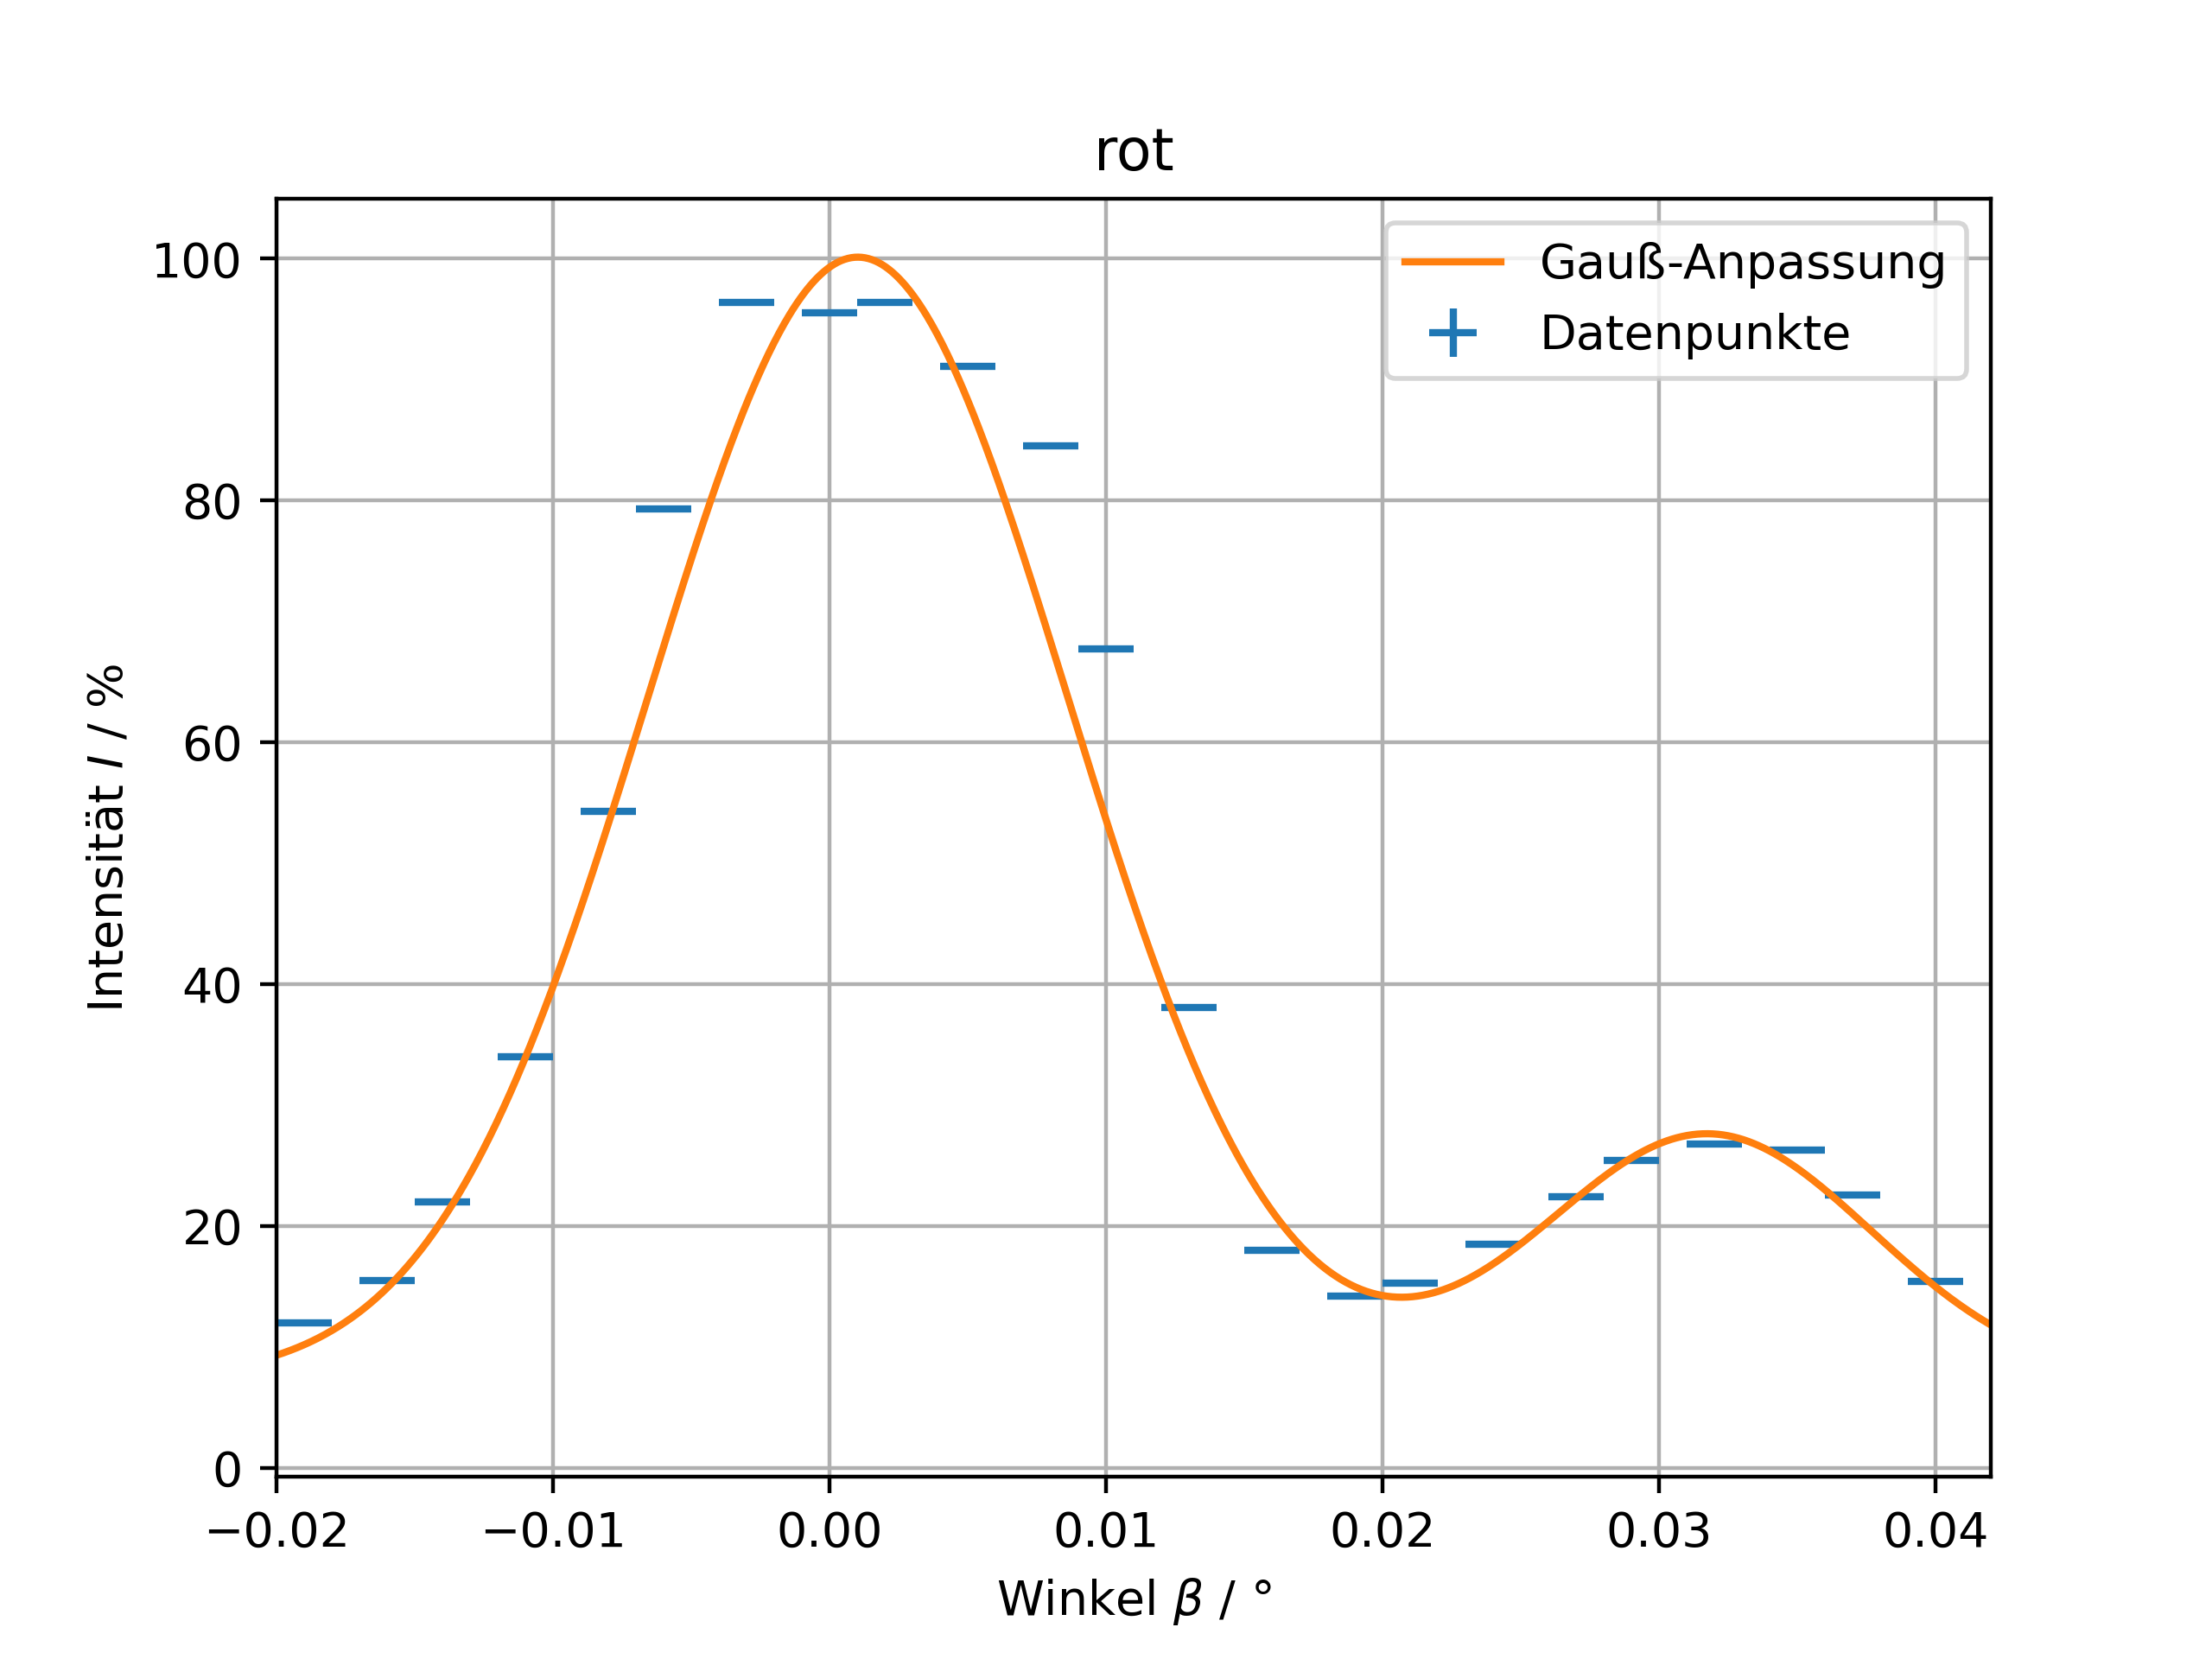
\includegraphics[width=\linewidth]{../figs/rot_fit}
        \caption{$\mathrm{H_{\alpha}}$-Linie}
    \end{subfigure}
    \begin{subfigure}{0.45\textwidth}
        \centering
        \includegraphics[width=\linewidth]{../figs/türkis_fit}
        \caption{$\mathrm{H_{\beta}}$-Linie}
    \end{subfigure}
    \begin{subfigure}{0.45\textwidth}
        \centering
        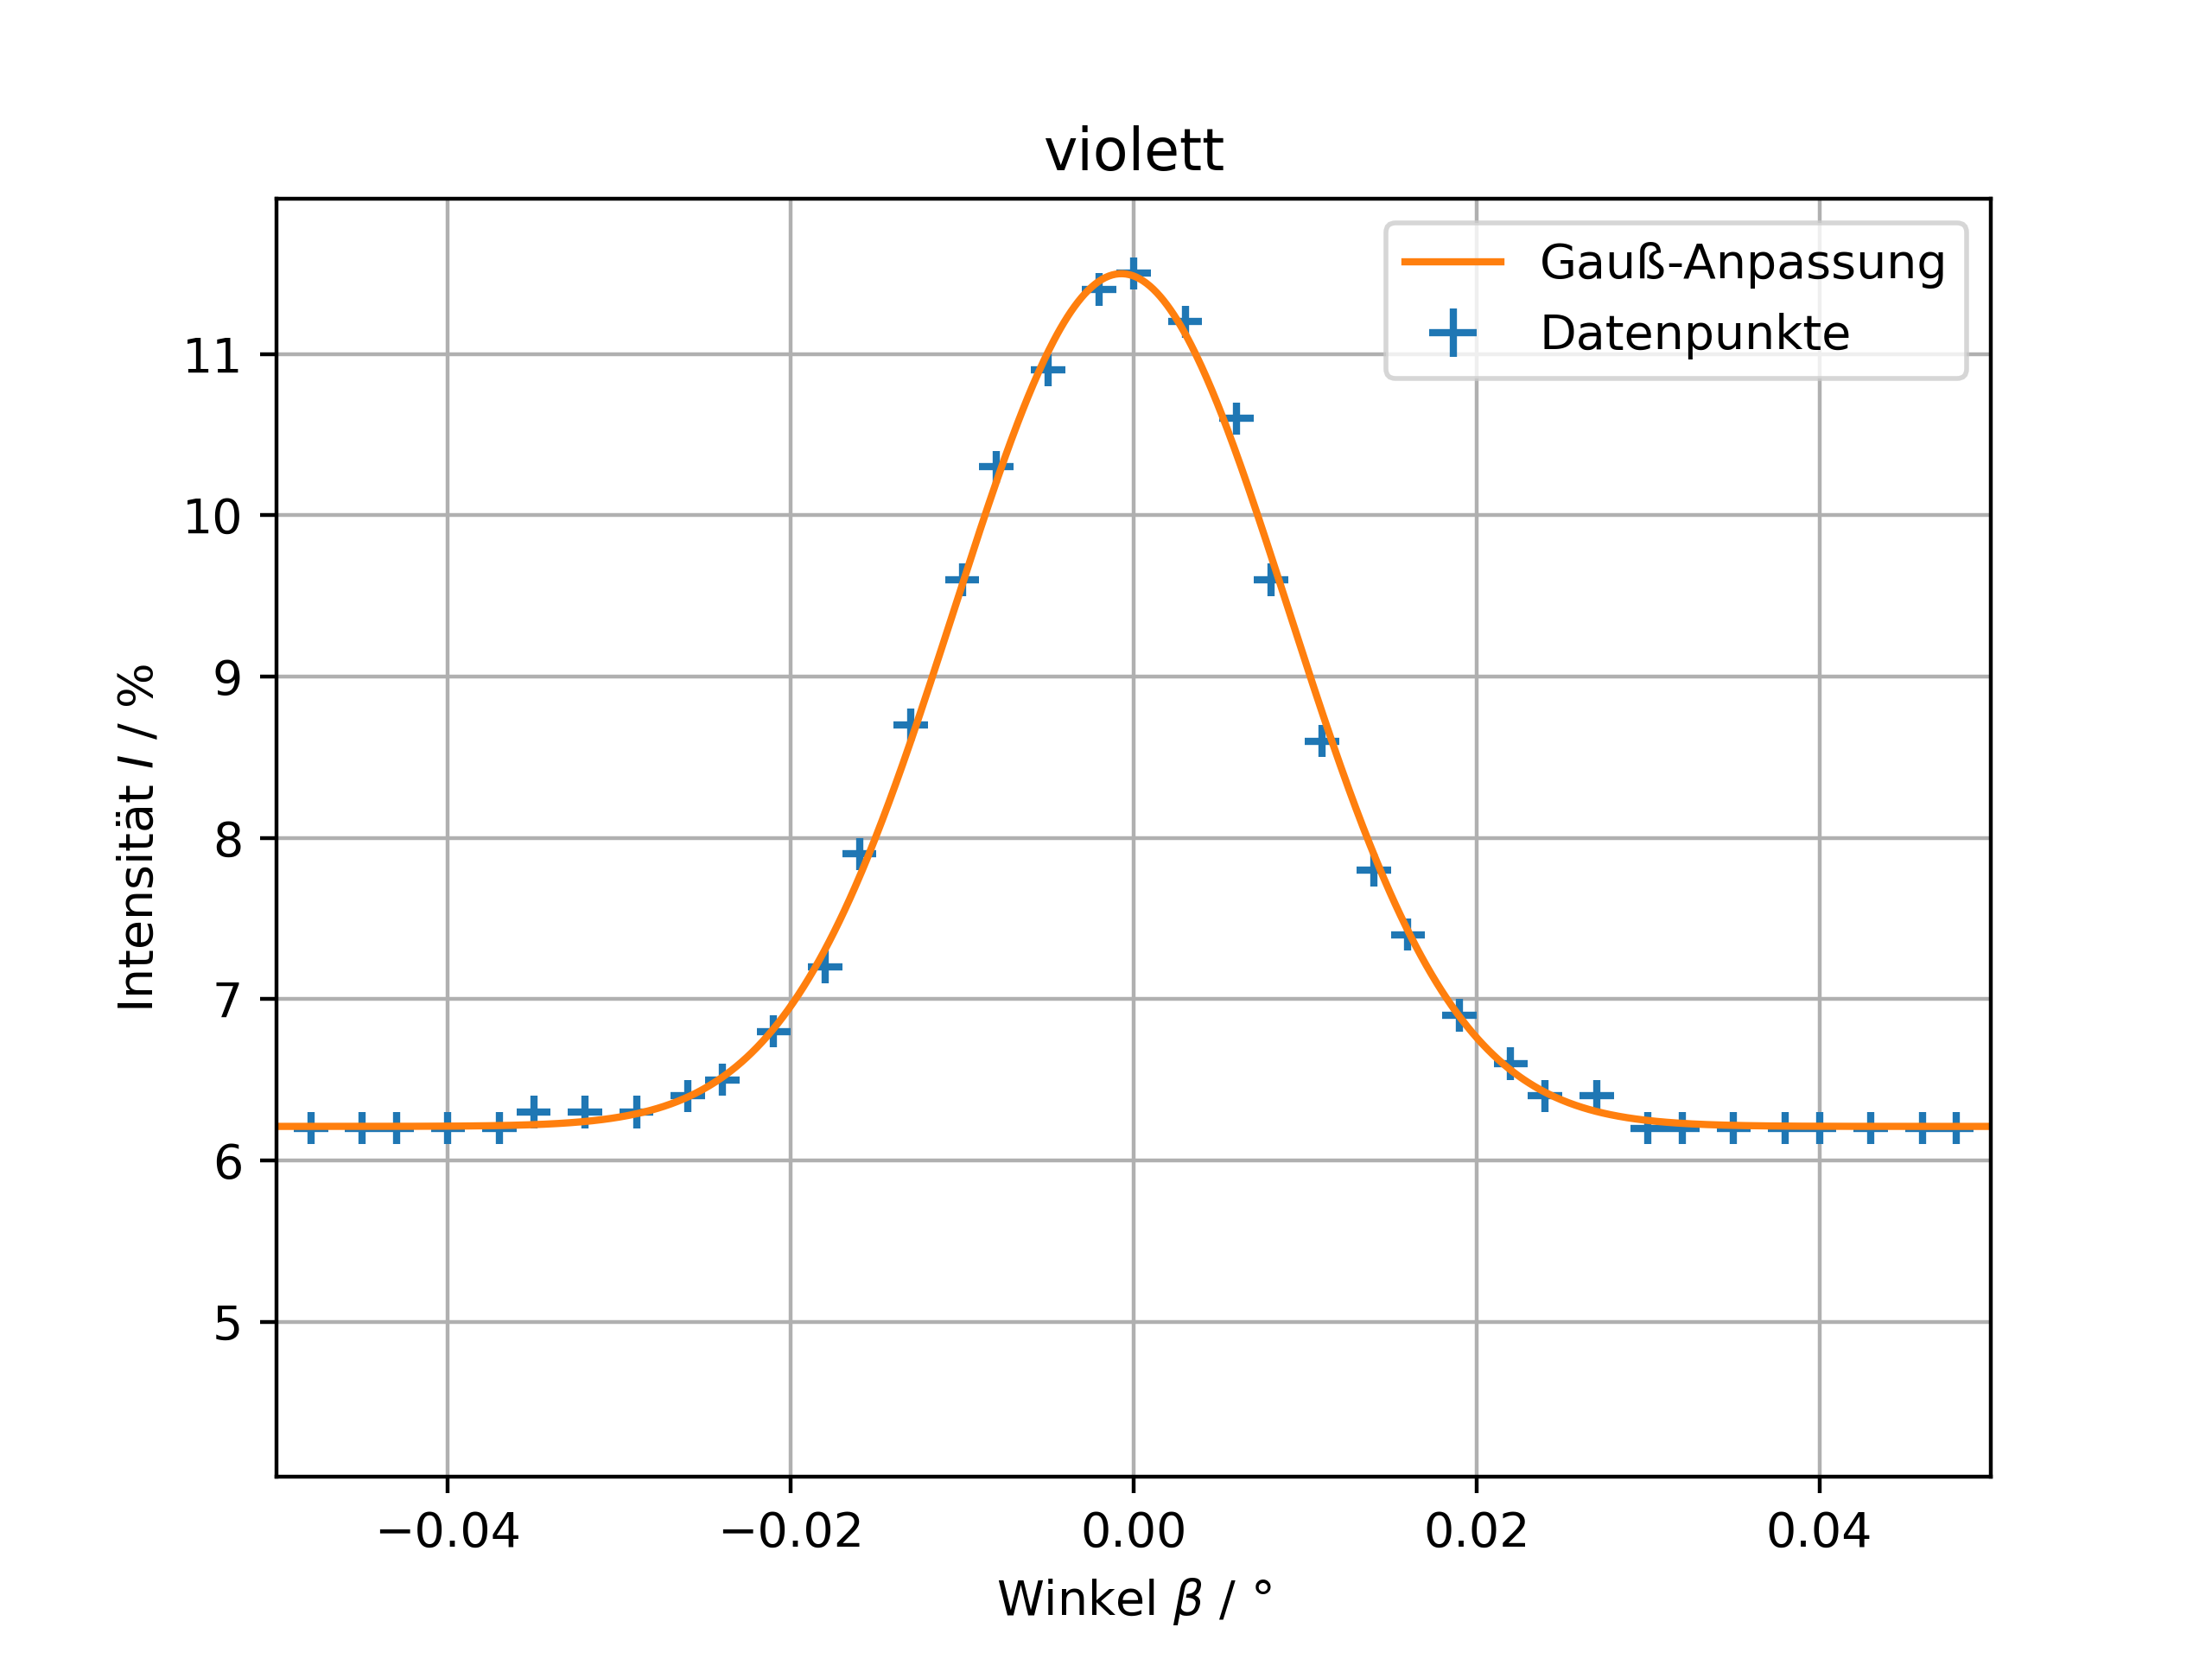
\includegraphics[width=\linewidth]{../figs/lila_fit}
        \caption{$\mathrm{H_{\gamma}}$-Linie}
    \end{subfigure}
    \caption{Mit der CCD-Kamera aufgenommene Intensitätsverteilungen der beobachteten Balmer-Spektrallinien inklusive Isotopieaufspaltung}\label{fig:exp_fits}
\end{figure}
\begin{table}[H]
    \centering
    \caption{Anpassungsparameter der Überlagerung zweier Gauß-Kurven}
    \begin{tabular}{c|c|c|c|c|c|c|c}
            & $A_1$ / \% & $\beta_1 \cdot 10^{-3}$ / \unit{\degree} & $\sigma_1 \cdot 10^{-3}$ / \unit{\degree} & $A_2$ / \% & $\beta_2 \cdot 10^{-3}$ / \unit{\degree} & $\sigma_2 \cdot 10^{-3}$ / \unit{\degree} & $O$ / \% \\
        \hline
        $\mathrm{H_{\alpha}}$ & 93 $\pm$ 5 & 1,0 $\pm$ 0,5 & 7,6 $\pm$ 0,8 & 20 $\pm$ 5 & 32 $\pm$ 1 & 5,9 $\pm$ 1,2 & 7 $\pm$ 5 \\
        $\mathrm{H_{\beta}}$ & 10 $\pm$ 1 & $-1$,4 $\pm$ 0,4 & 4,5 $\pm$ 0,3 & 1,2 $\pm$ 0,2 & 17 $\pm$ 1 & 3,2 $\pm$ 0,6 & 5,4 $\pm$ 0,1 \\
        $\mathrm{H_{\gamma}}$ & 5,3 $\pm$ 0,3 & $-$0,72 $\pm$ 0,11 & 9,7 $\pm$ 0,1 & 1 $\pm$ 0 & $-$0,4 $\pm$ 0,0 & 0,001 $\pm$ 0,000 & 6,21 $\pm$ 0,01
    \end{tabular}\label{tab:exp_fits}
\end{table} Bei der violetten $\mathrm{H_{\gamma}}$-Linie ist keine Isotopieaufspaltung zu erkennen, da (wie bereits auch schon zuvor) diese bei der Versuchsdurchführung
nicht aufgelöst werden konnte. Ein Grund dafür ist, dass der Versuchsaufbau nicht ganz präzise justiert war. Außerdem ist es möglich, dass die Intensität der Linie bzw. Aufspaltung zu gering war, da
der Spalt für eine schärfere Linie möglichst geschlossen werden musste. Weiterhin war eventuell das Projektionsobjektiv nicht ganz optimal auf die CCD-Kamera eingestellt. Bei der verwendeten Methode zur Anpassung der Überlagerung von zwei Gauß-Kurven ist die sogenannte \enquote{Residual variance} ein Maß für
die Güte der Anpassung (je näher an $0$, desto besser). Für die Anpassung an die $\mathrm{H_{\alpha}}$-Linie ist diese 2,56, für die Anpassung an die $\mathrm{H_{\beta}}$-Linie 1,31
und für die Anpassung an die $\mathrm{H_{\gamma}}$-Linie 0,15. Alle Anpassungen sind ausreichend gut gelungen. Es soll noch angemerkt werden, dass die Unsicherheiten für die Anpassungsparameter
der zweiten Gauß-Kurve an die $\mathrm{H_{\gamma}}$-Linie praktisch verschwinden, da das Programm hier aufgrund der fehlenden Auflösbarkeit der Isotopieaufspaltung effektiv nur
die erste Gauß-Kurve anpassen muss.\newline
\indent Die Winkel-Aufspaltung berechnet sich nun nach $\Delta \beta = \beta_2 - \beta_1$, wobei die Unsicherheit durch $\delta (\Delta \beta) = \sqrt{(\delta \beta_2)^2 + (\delta \beta_1)^2}$
gegeben ist. Für die Aufnahme der Messwerte mit der CCD-Kamera war $\omega_{\mathrm{G}}$ für die einzelnen Spektrallinien so eingestellt wie schon bei der Messung mit dem Okular, sodass auch die Ausfallswinkel $\beta$ gleich sind.
Die Isotopieaufspaltung wird nun erneut mit \ref{eq:isotopieaufspaltung} und der zugehörigen Unsicherheit berechnet. Die Ergebnisse sind in \cref{tab:aufspaltung_balmer_2} dargestellt.
\begin{table}[H]
    \centering
    \caption{Mit der CCD-Kamera bestimmte Isotopieaufspaltung der Balmer-Spektrallinien}
    \begin{tabular}{c|c|c|c|c}
        Spektrallinie & ($\Delta \beta \pm \SI{0,001}{\degree}$) / \unit{\degree} & $\Delta \lambda$ / \unit{\nano \meter} & $\delta (\Delta \lambda)$ / \unit{\nano \meter} & $\Delta \lambda_{\mathrm{Lit}}$ / \unit{\nano \meter} \\
        \hline
        $\mathrm{H_{\alpha}}$ & 0,031 & 0,174 & 0,007 & 0,19 \\
        $\mathrm{H_{\beta}}$ & 0,018 & 0,121 & 0,007 & 0,14 \\
        $\mathrm{H_{\gamma}}$ & / & / & / & 0,09
    \end{tabular}\label{tab:aufspaltung_balmer_2}
\end{table} Auch hier wurden gute Ergebnisse erzielt, da die Literaturwerte in der 3-$\sigma$-Umgebung der experimentell bestimmten Werte liegen. Die geringen Abweichungen kommen durch
den nicht perfekt justierten Versuchsaufbau zustande. Leider konnte auch mit dem Computer-Programm die $\mathrm{H_{\gamma}}$-Linie nicht scharf genug aufgelöst werden, um
die Isotopieaufspaltung zu beobachten, weshalb hier keine Auswertung der Isotopieaufspaltung möglich ist.

\subsubsection{Bestimmung der Rydberg-Konstanten}\label{subsubsec:rydberg}
Die Rydberg-Konstante kann nun aus den experimentell bestimmten Wellenlängen der vermessenen Balmer-Spektrallinien mit der Formel (entnommen aus \cite{balmer_handblatt})
\begin{equation*}
    \frac{1}{\lambda} = R_{\infty} \left(\frac{1}{4} - \frac{1}{n^2}\right)
\end{equation*} bestimmt werden. Diese Gleichung lässt sich als Geraden-Gleichung mit $y = \frac{1}{\lambda}$ und $x = \left(\frac{1}{4} - \frac{1}{n^2}\right)$
auffassen. Für die Unsicherheit der $y$-Werte gilt $\delta y = \frac{\delta \lambda}{\lambda^2}$. Die Geraden-Anpassung ist in \cref{fig:geraden_fit_rydbergkonstante}
dargestellt. Der Anpassungsparameter liefert die Rydberg-Konstante $R_{\infty} = \SI{1,110(2)e7}{\frac{1}{\meter}}$.
Der Literaturwert (entnommen aus \cite{Demtröder:829119}) $R_{\infty,\mathrm{Lit}} = \SI{1,096e7}{\frac{1}{\meter}}$ liegt außerhalb der 3-$\sigma$-Umgebung des experimentell bestimmten Wertes.
Dies liegt jedoch auch daran, dass die Unsicherheit vergleichsweise klein ist. Der Wert liegt trotzdem in dem richtigen Bereich. Vorhandene Abweichungen kommen dadurch zustande,
dass die Wellenlängen der Balmer-Spektrallinien nicht exakt bestimmt wurden.
\begin{figure}[H]
	\centering
	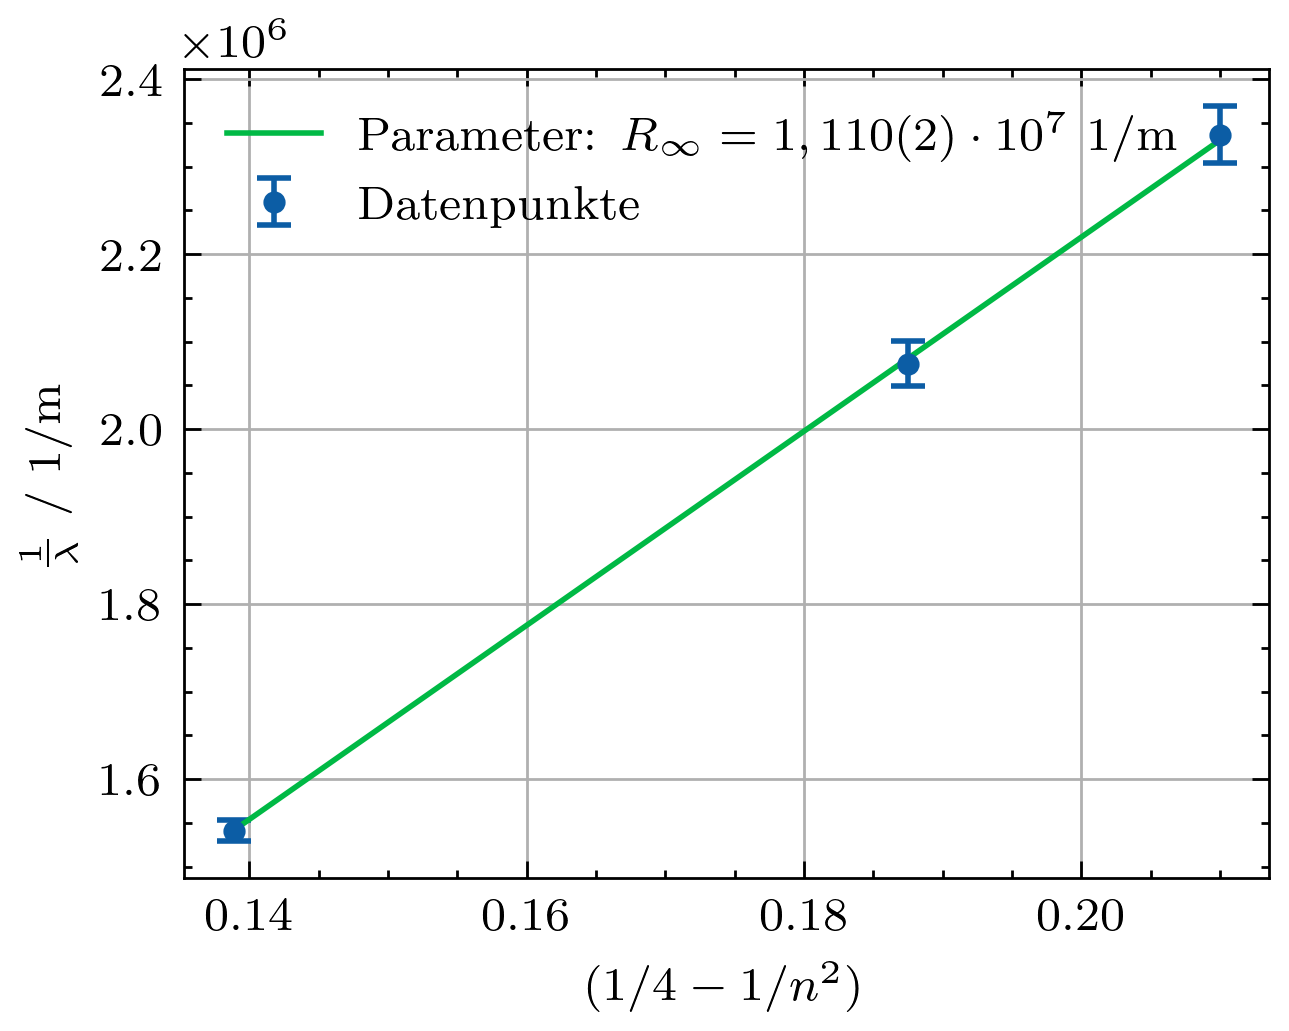
\includegraphics[width=0.8\linewidth]{../figs/rydbergkonstante_fit.png}
	\caption{Geraden-Anpassung zur Bestimmung der Rydbergkonstanten}
	\label{fig:geraden_fit_rydbergkonstante}
\end{figure}
\subsubsection{Bestimmung des Planckschen Wirkungsquantums}
Nach \cite{balmer_handblatt} lässt sich das Plancksche Wirkungsquantum über die soeben experimentell bestimmte Rydberg-Konstante wie folgt bestimmen:
\begin{equation*}
    h = \sqrt[3]{\frac{m_{\mathrm{e}}e^4}{8 \epsilon_0^2 R_{\infty} c}} .
\end{equation*} Hierbei ist $m_e$ die Elektronenmasse, $e$ die Elementarladung, $\epsilon_0$ die elektrische Feldkonstante und $c$ die Lichtgeschwindigkeit.
Diese Werte werden \cite{Demtröder:829119} entnommen. Die zugehörige Unsicherheit berechnet sich mit $\delta h = \frac{1}{3} \sqrt[3]{\frac{m_e e^4}{8 \epsilon_0^2 R_{\infty}^4 c}} \delta R_{\infty}$.
Damit ergibt sich für das Plancksche Wirkungsquantum:
\begin{equation*}
    h = \SI{6,600(4)e-34}{\joule \second} .
\end{equation*} Auch hier ist die Unsicherheit sehr klein, weshalb der Literaturwert für das Planscke Wirkungsquantum ($h = \SI{6,626e-34}{\joule \second}$)
außerhalb der 3-$\sigma$-Umgebung des experimentell bestimmten Wertes liegt. Dennoch ist das Ergebnis bis auf die erste Nachkommastelle genau,
weshalb ein gutes Ergebnis erzielt wurde. Der hier bestimmte Wert für das Plancksche Wirkungsquantum stimmt auch im Rahmen der Unsicherheiten
mit dem bestimmten Wert des Versuchsteils zum photoelektrischen Effekt überein, da bei diesem eine wesentlich größere Unsicherheit vorhanden ist.

\subsubsection{Weitere Überlegungen}

Bei der Versuchsdurchführung wurden bei der Betrachtung der Balmer-Linien noch weitere Spektrallinien im Hintergrund erkannt. Das Auftreten dieser
zusätzlichen Spektrallinien ist dadurch zu erklären, dass die Balmer-Lampe eine Gasentladung im Wasserdampf erzeugt, sodass
sich zusätzlich zum Wasserstoff (und Deuterium) noch Sauerstoff in der Lampe befindet, welcher zusätzlich schwache Linien vom roten bis grünen
Spektralbereich erzeugt. Außerdem kann es eventuell passsieren, dass bei dem Herstellungsprozess weitere Fremdatome in die Lampe geraten, sodass
der Wasserstoff bzw. das Deuterium in der Lampe nicht rein ist.\newline
\indent Die natürliche Linienbreite (welche durch die Energie-Zeit-Unschärfe bestimmt wird) wird durch den Doppler-Effekt (die Atome in der Balmer-Lampe bewegen sich in unterschiedliche Richtungen)
verbreitert. Nun soll diese Doppler-Verbreiterung der Linien abgeschätzt werden, welche mit folgender Formel (entnommen aus \cite{Demtröder:829119}) bestimmt werden kann:
\begin{equation*}
    \Delta \lambda_{\mathrm{D}} = \frac{\lambda}{c} \sqrt{\frac{8 k_{\mathrm{B}} T \ln(2)}{m}} .
\end{equation*} Die Unsicherheit berechnet sich gemäß
\begin{equation*}
    \delta (\Delta \lambda_{\mathrm{D}}) = \frac{\delta \lambda}{c} \sqrt{\frac{8 k_{\mathrm{B}} T \ln(2)}{m}} .
\end{equation*} Hier ist die Temperatur der Balmer-Lampe in \cite{skript} mit $T = \SI{1000}{\kelvin}$ angegeben. Die Masse von Wasserstoff H entspricht $1 \mathrm{u} = \SI{1,66e-27}{\kilogram}$
und die von Deuterium D etwa $2 \mathrm{u} = \SI{3,32e-27}{\kilogram}$. Die Boltzmann-Kostante wird \cite{Demtröder:829119} entnommen. Die abgeschätzten Werte sind in \cref{tab:doppler}
dargestellt.
\begin{table}[H]
    \centering
    \caption{Abschätzung der Doppler-Verbreiterung der Balmer-Spektrallinien}
    \begin{tabular}{c|c|c|c|c|c}
        Spektrallinie & $\lambda$ / \unit{\nano \meter} & $\Delta \lambda_{\mathrm{D}}(\mathrm{H})$ / \unit{\nano \meter} & $\delta (\Delta \lambda_{\mathrm{D}}(\mathrm{H}))$ / \unit{\nano \meter} & $\Delta \lambda_{\mathrm{D}}(\mathrm{D})$ / \unit{\nano \meter} & $\delta (\Delta \lambda_{\mathrm{D}}(\mathrm{D}))$ / \unit{\nano \meter} \\
        \hline
        $\mathrm{H_{\alpha}}$ & 649 & 0,0147 & 0,0002 & 0,0104 & 0,0001 \\
        $\mathrm{H_{\beta}}$ & 482 & 0,0109 & 0,0002 & 0,0077 & 0,0001 \\
        $\mathrm{H_{\gamma}}$ & 428 & 0,0097 & 0,0002 & 0,0068 & 0,0001
    \end{tabular}\label{tab:doppler}
\end{table} Ein Vergleich mit Literaturwerten ist hier nicht nötig, da die verwendete Formel der Literatur selber entnommen ist und die eingesetzten
Wellenlängen im Rahmen der Unsicherheiten mit den Wellenlängen der Literatur übereinstimmten.\newline
\indent Die natürliche Linienbreite wird nach \cite{Demtröder:829119} mit $\Delta \nu = \frac{1}{2 \pi \tau}$ bestimmt, wobei $\tau$
die typische mittlere Lebensdauer optischer Übergänge ist. Diese beträgt nach \cite{Demtröder:829119} \SI{1e-8}{\second}.
Mit $\frac{\Delta \nu}{\nu} = \frac{\Delta \lambda}{\lambda}$, $c = \lambda \nu$ und einer Wellenlänge in etwa der Mitte der betrachteten Balmer-Spektrallinien
von \SI{500}{\nano \meter} folgt:
\begin{equation*}
    \Delta \nu \approx \SI{16}{\mega \hertz} ,
\end{equation*}
\begin{equation*}
    \Delta \lambda = \lambda^2 \frac{\Delta \nu}{c} \approx \SI{1,33e-5}{\nano \meter} .
\end{equation*} Im Vergleich mit der Doppler-Verbreiterung fällt auf, dass die natürliche Linienbreite um etwa 3 Größenordnungen
kleiner ist. Somit ist für die Messung nur die Doppler-Verbreiterung der Spektrallinien entscheidend.\newline
\indent Die Doppler-Verbreiterung kann auch aus den Gauß-Anpassungen der mit der CCD-Kamera aufgenommenen Messwerte bestimmt werden, da sich die
Doppler-Verbreiterung auf die Halbwertsbreite einer an die Spektrallinie angepassten Gauß-Kurve bezieht.
Dafür wird die Standardabweichung $\sigma_1$ bzw. $\sigma_2$ benötigt, je nachdem ob die Doppler-Verbreiterung der Wasserstoff-Linie oder der
Deuterium-Linie bestimmt werden soll. Die Werte für die Standardabweichungen der Gauß-Kurven werden aus \cref{tab:exp_fits} entnommen.
Die Halbwertsbreite einer Gauß-Kurve berechnet sich bekanntlich gemäß
\begin{equation*}
    \Delta \beta_{1/2} = 2 \sqrt{2 \ln(2)} \sigma_{1/2}
\end{equation*} mit der Unsicherheit
\begin{equation*}
    \delta (\Delta \beta_{1/2}) = 2 \sqrt{2 \ln(2)} \delta \sigma_{1/2} .
\end{equation*} Die entsprechende Doppler-Verbreiterung kann mit \ref{eq:isotopieaufspaltung} und der zugehörigen Unsicherheit berechnet werden. Die Ergebnisse sind in \cref{tab:doppler2} dargestellt.
\begin{table}[H]
    \centering
    \caption{Bestimmung der Doppler-Verbreiterung der Balmer-Spektrallinien aus den Halbwertsbreiten der angepassten Gauß-Kurven}
    \begin{tabular}{c|c|c|c|c|c|c}
        Spektrallinie & $\Delta \beta_1$ / \unit{\degree} & $\delta (\Delta \beta_1)$ / \unit{\degree} & $\Delta \beta_2$ / \unit{\degree} & $\delta (\Delta \beta_2)$ / \unit{\degree} & $\Delta \lambda_{\mathrm{D}}(\mathrm{H}) \pm \num{0,0001}$ / \unit{\nano \meter} & $\Delta \lambda_{\mathrm{D}}(\mathrm{D}) \pm \num{0,0001}$ / \unit{\nano \meter} \\
        \hline
        $\mathrm{H_{\alpha}}$ & 0,018 & 0,002 & 0,014 & 0,003 & 0,0264 & 0,0205 \\
        $\mathrm{H_{\beta}}$ & 0,011 & 0,001 & 0,008 & 0,002 & 0,0388 & 0,0276 \\
        $\mathrm{H_{\gamma}}$ & 0,023 & 0,001 & / & / & 0,0954 & /
    \end{tabular}\label{tab:doppler2}
\end{table} Die Unsicherheit für die experimentell bestimmte Doppler-Verbreiterung wurde hier zusätzlich etwas größer abgeschätzt als eigentlich berchnet, da die Unsicherheit ansonsten verglichen
mit den minimalen systematischen Unsicherheiten des Versuchsaufbaus zu klein ist. Werden die experimentell bestimmten Werte für die Doppler-Verbreiterung
aus \cref{tab:doppler2} mit den theoretisch abgeschätzten Werten aus \cref{tab:doppler} verglichen, so fällt auf, dass die experimentell bestimmten Werte
bis zu einer Größenordnung breiter sind. Dies legt nahe, dass der Versuchsaufbau nicht optimal justiert war. Außerdem hätte die Spaltbreite
besser eingestellt werden müssen. Dies war jedoch in der vorgegebenen Durchführungszeit nicht zu erreichen, da eine so genaue Justierung viel Zeit benötigt.
Es musste schließlich der Fokus darauf gelegt werden, die Spektrallinien überhaupt ausreichend gut genug zu erkennen und vermessen zu können.\newline
\indent Das Auflösungsvermögen des verwendeten Reflexionsgitters berechnet sich nach \cite{Demtröder:829122} ungefähr nach $A = \frac{\lambda}{\Delta \lambda} = m N$,
wobei $\lambda$ die beobachtete Wellenlänge ist, $\Delta \lambda$ die gerade noch auflösbare Wellenlängendifferenz, $m$ die Beugungsordnung und $N$ die Anzahl
der ausgeleuchteten Spalte. Bei der Versuchsdurchführung wurde nur die erste Beugungsordnung beobachtet, womit $m=1$ ist. Das Auflösungsvermögen ist gegeben durch:
\begin{equation*}
    A = N = \frac{\text{beleuchtete Gitterbreite}}{\text{Gitterkonstante}} = \frac{d}{g}, \quad \delta A = \frac{d}{g^2} \delta g .
\end{equation*} In der Versuchsanleitung \cite{skript} ist die beleuchtete Gitterbreite mit $d = \SI{25}{\milli \meter}$ angegeben, womit
für das Auflösungsvermögen des Gitters folgt:
\begin{equation*}
    A = \num{61400(800)} .
\end{equation*} Die gerade noch auflösbare Wellenlängendifferenz berechnet sich nun mit $\Delta \lambda = \lambda \frac{g}{d}$ und $\delta (\Delta g) = \lambda \frac{\delta g}{d}$
(hier wird wieder eine Wellenlänge von $\lambda = \SI{500}{\nano \meter}$ eingesetzt):
\begin{equation*}
    \Delta \lambda = \SI{8,1(1)e-12}{\meter} .
\end{equation*} Somit wäre es mit diesem Gitter bei voller Ausleuchtung möglich gewesen, die Isotopieaufspaltung vollständig aufzulösen.
Jedoch wurde das Gitter nicht voll ausgeleuchtet, wodurch das tatsächliche Auflösungsvermögen des Gitters bei der Versuchsdurchführung geringer war
als hier berechnet. Auch war die Spaltbreite nicht bei jeder Messung optimal eingestellt, was dazu geführt  hat,
dass die Isotopieaufspaltung nicht immer scharf zu erkennen war.